第0講では、プログラミングに関係するパソコンの基礎知識を説明する。これから車の運転を習おうという人がブレーキやアクセルとは何だと訊くことはまずないだろう。だが、プログラミングの場合、ブレーキやアクセルに相当する部分を知らずに学ぼうということが少なくない。そこで、ここではそれらの必要最小限の説明を付しておく。もちろん、知っているならば読み飛ばしてもらって良い。
\\ \\ 
ここでは、情報数学の一環として、まず記数法について説明する。次いで、パソコンの仕組みについて触れ、最後に学習環境の構築について記しておく。
\section{記数法とコンピュータ}
我々が物を数える際には手の10本の指を用いる。ここから物を数える位取りとして、指がいっぱいになったら位を1増やすということで\textbf{10進法}\index{じゅっしんほう@10進法}(decimal system)が生まれた。10進法とは、10(十、ten)毎に位がひとつ上がるような数え方であり、我々が普段使っている数の表記法である。10進法により表された数のことを\textbf{10進数}\index{じゅっしんすう@10進数}(decimal digit)と呼ぶ。

一方、コンピュータはON/OFFで表すという事から、2つの状態(=2つの指)を持つといえる。このことから、コンピュータは2毎に位がひとつ上がり、0,1,10,11,...と数える\textbf{2進法}\index{にしんほう@2進法}(binary system)を中心に使っている。
\\ \\ 
これらのような、数の表記にあたりどのようにして位をとるかの方法を\textbf{位取り記数法}\index{くらいどりきすうほう@位取り記数法}(positional notation)あるいは単に\textbf{記数法}\index{きすうほう@記数法}と呼ぶ。ここでは、記数法の一般論と、コンピュータでよく使われる記数法の利用について学ぶ。

\subsection{記数法の一般論}
先までの例と同様に、指の本数から考えよう。指が$n(\ge2)$本しかないと仮定する。このときは、$n$本がいっぱいになったら次の位に移る。たとえば、指が3本しかなければ、3になったら次の位に移るようにして数えることができる。

一般の自然数$n$に対して、$n$進法とは、$n$を位取りにする方法である。つまり、数えていって、$n$に達する毎に上の位に移るという事である。

例えば、123という数字を考えよう。これは、123個の1であるが、同時に12個の10と3個の1である。更に分ければ、1個の100と2個の10と3個の1と分かれる。つまり、$10^k$の束がいくつあるかを数え、それが10個に達したら$10^{k+1}$を1増やす。これによって、各位は$10^{k+1}$の束にならない余りとなる\footnote{これは後に学ぶ記数法の変換と桁わけの意味を理解するのに重要である。}。

上記に従って位取りをしてみよう。10進法では、小数点の直上を$10^0$とし、その上の桁を$10^1,10^2,\cdots$、小数点以下を$10^{-1},10^{-2},\cdots$としている。この10を$n$に変えたのが$n$進法である。たとえば、2進法における11111は$2^4\times1+\cdots+2^0\times1=31$である。
\\ \\ 
$n$進法で使われる数字は、$n$種類ある。2進法なら0と1だし、10進法なら0, 1, 2, 3, 4, 5, 6, 7, 8, 9であり、16進法の場合は0, 1, 2, 3, 4, 5, 6, 7, 8, 9, a, b, c, d, e, fである\footnote{アルファベットは大文字を用いることもある。C言語ではどちらを用いても構わない。}。

位取り記数法は筆算と相性がよく、四則演算は何れも10進法の場合同様に筆算を用いて計算することができる。これにより、記数法を変更しても、計算は苦労なくできるはずである。(但し、後に学ぶ方法を用いて、10進法に一度変換してから行なっても問題はない)。

何進法であるかを明確にするときには、数字の右下に$33_{(n)}$のように記す。たとえば、$101.1_{(2)}=5.5_{(10)}$である。

\subsection{記数法の変換}
ここでは、記数法を変換する方法について考えよう。まず、一般論として10進法を介して変換する方法を述べ、次いでコンピュータでよく用いられる2進/8進/16進の直接変換法を見てみる。
\minisec{10進法との相互変換}
$n$進法から10進法への変換はどのように行うだろうか。これは$n$進法の仕組みを考えてみればわかる。

$n^k$の位が$a_k$であるような数字$A$の10進法での値は次のように求められる。
\begin{itembox}[l]{$n$進法から10進法への変換}
$n^k$の位が$a_k$であるような数字$A_{(n)}$は、10進法において
\begin{equation*}
A_{(10)}=\sum_{k}a_k\times n^k
\end{equation*}
と計算できる。
\end{itembox}
これは、$n$進法の定義を考えれば直接出てくる方法である。
\\ \\ 
逆に、10進法から$n$進法に変える場合は、どうすればよいだろうか。

1つには、単に「取り尽くす」方法がある。つまり、$n^k$のうち、元の数を超えない最大のものを見つけ、その数で元の数を割った商を$n^k$の位にし、余りについて$n^{k-1}$で割り…と繰り返すのである。特に、小数点がある場合はこの方法を利用すると楽である。

だが、この計算はやや面倒に感じることもあろう。そこで、主に整数向けであるが、先に書いた位取りの考えを用いる方法がある。

$n^k$の位が$a_k$であるという事は、$n^k$で割った後に、小数点以下を切り捨て、$n$に対する剰余を取ると$a_k$になる、という事である。例えば、10進法で100の位の数字を出したいとすれば、100で割って10による余りを取れば良い。これと同じ性質が一般の$n$進法にも成立する。この性質を利用し、次のような手順を踏んで記数法を変換できる。
\begin{itembox}[l]{10進法から$n$進法への変換}
\begin{enumerate}
\item 変換したい10進数を$n$で割り、その余りをメモする。
\item これを、商が0になるまで繰り返す。
\item メモした余りを逆から順に並べると$n$進数での表記になる。
\end{enumerate}
\end{itembox}

この方法は、$n$進有限小数で表せる場合、$n$の整数乗をかけてから実行することで有限小数の場合にも適用できる。
\\ \\ 
一例として、12.25$_{(10)}$を8進法に変換してみよう。

まず、これを8倍してやれば、98になる。8倍するというのは8進法で1桁上にあげたことを意味するので、最後に1桁下げることで辻褄を合わせる。

次いで、98を8で割っていく。順に書くと
\begin{eqnarray*}
98/8&=&12\ \cdots 2\\
12/8&=&1\ \cdots 4\\
1/8&=&0\ \cdots 1
\end{eqnarray*}
となるので、これを下側から順に読んで、142となる。1桁上げていることを考慮すれば、12.25$_{(10)}$=14.2$_{(8)}$である。逆に変換してみれば正しいことが明らかだろう。
\\ \\ 
いくつかの数を変換してみればわかるが、10進整数は他の記数法でも整数である。一方、ある記数法で有限小数であるからと言って他の記数法で有限小数であるとは限らない。例えば、1/3は、10進法では無限小数だが、3進法であれば0.1$_{(3)}$とシンプルに表せる。

\minisec{2進/8進/16進の直接変換}
コンピュータの世界では、内部的な処理の関連で2進法をよく使うが、これを見やすくするために8進法や16進法が使われる。また、添字形式はコンピュータで表現しづらいため、8進法は0をつけて025などと、16進法は0xないし0Xをつけて、0x3aや0X5Bなどと記す(xの大小と英字の大小が対応している)。以下では、この記法を用いて記す。
\\ \\ 
2進法を見やすくするために8/16進法を使うと書いたが、これは、2進法を3/4桁毎にまとめたものが8/16進法だからである。

具体例を見てみよう。2進法で110010011111という数字を考える。まず、これを8進法に変換してみよう。

3桁ごとに分けて書けば110 010 011 111となる。ここで、一番下の3桁はそのまま8で割った余りである。次の3桁は、8で割り切れるが64では割り切れない部分である。同様に考えていけば、2進法3桁ごとに8進法1桁と同じ値を表していることがわかる。そこで、これを3桁ごとに10進法に直すのと同じ要領で計算すれば06237と変換できる。
\\ \\ 
これを今度は4桁ごとに分けてやると、1100 1001 1111となる。同じ要領で16進法に変換することができ、0xc9fとなる。
\\ \\ 
このように、2進法での表記は8/16進法に簡単に変換できる。逆に、8/16進法を用いて書いたものを2進法に直したいならば、各位を3/4桁の2進数に変換して並べれば良い。

例えば、0xbea2などという数字があった時、10進法を介すると大変だが、直接変換すれば、bは1011,eは1110,aは1010,2は0010なので、これを並べて1011111010100010と変換することができる。
\\ \\ 
一般に、$n$進法と$n^k$進法の間では、このように$k$桁毎の直接変換を行うことができる。実際に使うのは、2/8/16進法の間での直接変換ぐらいだろうが、知っておくと便利である。

\subsection{ビットとバイト}
コンピュータはどのようなデータも2進数で表している。この2進数1桁(あるいはその情報量)を1\textbf{ビット}\index{びっと@ビット}(bit,BInary digiTの略)という。このことから、例えば16bitの情報は、全部で$2^{16}=65536$通りあることがわかる。また、モデム回線の56kbpsや光ファイバーの100Mbpsといった回線速度の単位bpsはbit per secondの意味で、それぞれ56*1000ビット、100*1000*1000ビットの情報を1秒間にやり取りできることを示している\footnote{k(キロ)やM(メガ)は通常10$^3$や10$^6$である。だが、コンピュータの世界では$2^{10}$が1024で$10^3$に近いため、これを用いて表すこともある。コンピュータの世界でもこれらは混同されており、500GBと書かれたHDDを買ってきて接続すると、コンピュータ側では536GBと表示されるなどの違いが出ることもある。なお、混同をなくすために$2^{10}$を使っている場合には接頭辞の後ろにiをつけ、kiB(キビバイト)やMiB(メビバイト)として表すこともある。}。
\\ \\ 
だが、データの単位としてビットを使ってばかりいると大きくなるし、まとまりも悪い。また、13ビットの情報などは、先に書いたような8/16進表記もしづらい。そこで、16進法を使って簡単に表せるよう16進2桁=8bitの情報を1\textbf{オクテット}\index{おくてっと@オクテット}(octet)として扱うことになっている\footnote{鉛筆12本を1ダースとして数えるのと同じような感覚である。}。そして、データの大きさは通常、オクテットを用いて表す。だが、実際に聞くことがあるのはオクテットではなくてバイトであろう。

\textbf{バイト}(byte)は、一般的にはオクテットと同じ単位であり、1byte=1octet=8bitである\footnote{一般にbはbitを、BはByteを表す。従って、56kbpsと7kBpsは同じ速度である。}。但し、環境によっては1byteが1octetではない場合もある。この為、8bitであることを明確に示すための1octetという言い方が生まれたのである。なお、本書では特に断りない場合、1byte=1octetとする。

1byteは8bitであるので、1byteによって表せる情報は$2^8=256$通りあることがわかる。これだけあれば世界共通で使われる文字などを表すことができるため、これらの文字は\textbf{1バイト文字}\index{いちばいともじ@1バイト文字}と呼ばれている。

以上のように、Byteというのは2進法(=bit)から決められた単位であるので、その大きさを計算するためには、bitに直してやれば良い。

\section{パソコンの仕組み}
パソコンの仕組みについて、簡単に紹介しておく。
\subsection{パソコンを構成する装置}
パソコンは大きくいって次のような装置から構成されている。
\begin{itembox}[l]{コンピュータを構成する装置}
\begin{itemize}
\item \textbf{入力装置}\index{にゅうりょくそうち@入力装置}(input device):コンピュータ(や実行中のプログラム)にデータや情報、指示などを与えるための装置。キーボードやマウス、スキャナ・マイク等。
\item \textbf{出力装置}\index{しゅつりょくそうち@出力装置}(output device):コンピュータの計算結果などを何らかの形で出力する装置。ディスプレイ・スピーカー等。
\item \textbf{中央演算処理装置}\index{ちゅうおうえんざんしょりそうち@中央演算処理装置|see{CPU}}(\textbf{CPU}\index{CPU},Central Processing Unit):厳密には\textbf{論理演算装置}\index{ろんりえんざんそうち@論理演算装置}(arithmetic logic unit)と\textbf{処理装置}\index{しょりそうち@処理装置}(control unit)に分かれるが、実際にはこれらをまとめてCPUとして取り付けているのが普通である。コンピュータの演算や処理を行う、頭脳と言える装置である。
\item \textbf{主記憶装置}\index{しゅきおくそうち@主記憶装置}(main memory/main storage):後に示す補助記憶装置とあわせて\textbf{記憶装置}\index{きおくそうち@記憶装置}(memory/storage)と呼ばれる。揮発性(通電されなくなると記憶内容が消えてしまう)の記憶装置で、CPUから高速にアクセスすることができる部分である。これは、CPUが作業を行うための机のような役割を果たす装置である。これはC言語プログラミングで重要であるので、後でより詳らかにする。
\item \textbf{補助記憶装置}\index{ほじょきおくそうち@補助記憶装置}(external memory/external storage):先に記した主記憶装置とあわせて、記憶装置と呼ばれる。不揮発性(通電されなくなっても記憶内容が残っている)であり、CPUからのアクセス速度が主記憶装置より遅いが、安価で大容量である。HDDやSSDがこれに相当し、データ収納の役割を果たす。なお、補助記憶装置の一部を主記憶装置のようにみなし、主記憶装置で容量不足が起こった時などに用いることができるようにした技術として\textbf{仮想メモリ}\index{かそうめもり@仮想メモリ}がある\footnote{Linuxの場合、HDD上にswap領域と呼ばれる領域を作成し、その部分を仮想メモリとして用いる。Windowsでも、明確にswap領域としてパーティションを作ることはないが、この仕組みを使っている。USBフラッシュメモリによるReadyBoostもこの技術の一例である。}。
\end{itemize}
\end{itembox}

これらの、入力装置・出力装置・論理演算装置・制御装置・記憶装置をまとめて\textbf{コンピュータの5大装置}\index{ごだいそうち@5大装置}などという事もある。
\\ \\ 
これらの装置がどのようにしてデータを処理するかを見ていこう。

まず、CPUが入力装置に対して入力を受け付けるように制御する信号を出す。これによって入力装置は入力を受け付けるようになる。その後、データの入力が行われ、主記憶装置に保存される。これに対してCPUが適切に処理を行い、必要に応じて外部記憶装置に格納したり出力装置に渡して出力したりする。CPUは処理と共に、データの格納や出力、あるいは外部記憶装置からの読み出しなどの制御も行なっている。

以上に述べた装置の動作を図示したものが図\ref{fig0_1}である。
\begin{figure}[htb]
\centering
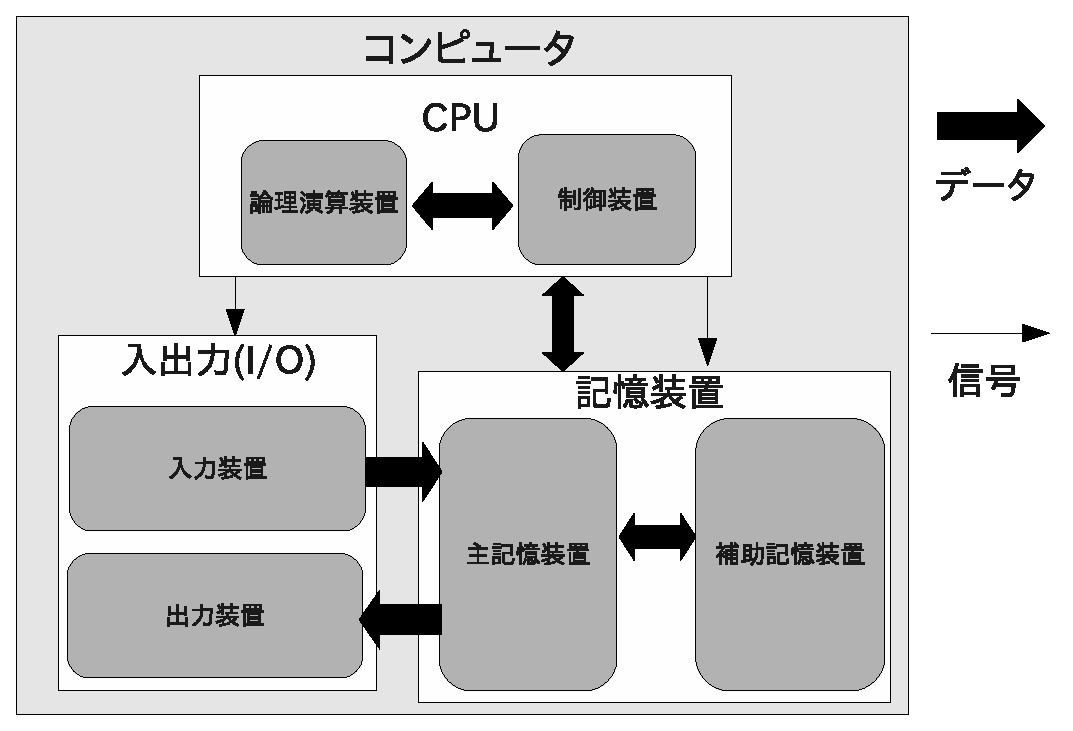
\includegraphics[width=0.9\linewidth,keepaspectratio]{fig0_1.eps}
\caption{コンピュータの装置間の動作}\label{fig0_1}
\end{figure}

\subsection{主記憶装置}
今後学んでいくC言語では、メモリをはじめとした主記憶装置について意識しないといけない場面が数多く出てくる。この為、主記憶装置については他の装置以上に深い理解が要求される。C言語そのものを学ぶ前に、主記憶装置への理解を深めておこう。
\minisec{主記憶装置の種類}
主記憶装置は、CPUからの距離に応じて大別される。

CPUはその最も近いところに\textbf{レジスタ}\index{れじすた@レジスタ}(register)と呼ばれる主記憶装置を持っており、これが一番高速に用いられる主記憶装置である。次いで、\textbf{キャッシュメモリ}\index{きゃっしゅめもり@キャッシュメモリ}(cache memory)と呼ばれる主記憶装置がある\footnote{さらに、キャッシュメモリ自体も近い順に1次、2次、3次と大別される}。そして、我々が一般に\textbf{メモリ}\index{めもり@メモリ}(memory)と呼んでいる主記憶装置(実際に区別するためには\textbf{メインメモリ}と呼ぶことが多い)があり、この3つによって主記憶装置が成り立っている。

このように3つに分けているのは、CPUから近ければ近いほど高速であるが、その分容量が減るためである。例えば、レジスタはメモリに比べるとずっと小さい。従って、必要に応じて、「どの主記憶装置を用いるべきか」も考慮しなければならない。

\minisec{RAM}
メインメモリは\textbf{RAM}\index{RAM}(Random Access Memory)とも呼ばれる\footnote{似た言葉に\textbf{ROM}\index{ROM}があるが、これはRead-Only Memoryの略で、一度書き込んだら書き換えられないような領域を指す。}。これは、前から順に「どこに書きこめばよいか」を探さなければならない\textbf{シーケンシャルアクセス}\index{しーけんしゃるあくせす@シーケンシャルアクセス}(sequential access)を用いると、メモリへのアクセス速度を損ねてしまうからである\footnote{なお、HDDは比較的シーケンシャルアクセスに近いアクセスで、目的のファイルを読み出すのに時間がかかる。一方、SSDはランダムアクセスの性能が高く、HDDより高速なアクセスを実現している。}。どこか空いているところを電気的にすぐに判定し、そこに書きこむようにする\textbf{ランダムアクセス}\index{らんだむあくせす@ランダムアクセス}を用いて速度を損ねることなく利用できるようにしているのである。

また、ランダムアクセスすると、メモリ全体の使われる頻度が均一になり、長持ちしやすいという利点もある。
\\ \\ 
メインメモリには、ここに述べたようにランダムアクセス方式を用いる。このため、RAMと呼んだ場合はメインメモリのことを指すのが一般的である。

\minisec{メモリの領域}
C言語を用いてプログラミングを行う場合、メモリの領域は次の4つに大別される。
\begin{itembox}[l]{Cにおけるメモリ領域}
\begin{itemize}
\item \textbf{プログラム領域}\index{ぷろぐらむりょういき@プログラム領域}:プログラムを実行するためのプログラムコードが置かれる領域。プログラムを実行したい場合、そのプログラムはメモリ上にロードされ、順次実行されることになる。このロードに使われる領域の事。
\item \textbf{静的領域}\index{せいてきりょういき@静的領域}:外部変数や静的変数といった、プログラムの実行中に変化しない(実行中ずっと寿命が保たれている)変数を格納する領域。寿命については後に学ぶ。
\item \textbf{スタック領域}\index{すたっくりょういき@スタック領域}:一般の変数、関数の引数や返却値、長い計算式の一時変数などが置かれる領域。
\item \textbf{ヒープ領域}\index{ひーぷりょういき@ヒープ領域}:プログラム中で動的にメモリが確保される場合に使われる領域。
\end{itemize}
\end{itembox}

自作のプログラムを実行したとしよう。実行されたプログラムは、まずプログラム領域にロードされる。この時、静的領域とスタック領域が割り当てられる。これらの大きさはプログラム実行中不変であるが、静的領域は領域内の使用量が実行中に変化しないのに対し、スタック領域では領域内の使用量が実行中に変化する。このことから、スタック領域の割り当ては「スタック領域をどれだけ使っていいか」という、限度の割り当てである。

以上でプログラムがロードされたら、このあとはプログラム領域の命令を順次読み取ってCPUが処理を実行する。この際、プログラム側が動的にメモリを確保したいと要求すればヒープ領域を用いることになる。

現状ではまだピンと来ない説明かもしれないが、本書を学んでいくうちに、必要に応じてここに戻ってきていただければ、理解できるだろう。

\minisec{メモリとアドレス}
メモリはランダムアクセスであるが、その場所がわからないと困る。そこで、メモリには\textbf{アドレス}\index{あどれす@アドレス}(address)という番号がふられており、これによってメモリ上に配置されているデータの場所が示される。

プログラミング言語を機械に近づけていくと、このアドレスを用いたメモリいじりが主体であることがわかる。逆に、近年生まれた「人間に近い」言語はアドレスいじりを直接目に見える形では行わない場合が多い。

ひとまずここでは、メモリの番地を表すアドレスという指標があるという事を知っておいていただきたい。

\minisec{スタック領域とヒープ領域の特徴}
先に説明したスタック領域とヒープ領域の特徴について、少し記しておく。
\\ \\ 
まず、ヒープ領域はある種の共通領域で、割り当てなどがないのに対し、スタック領域には割り当てがあるという点が違う。メモリが空いている時、ヒープ領域は空いている限り使うことができるが、スタック領域はいくらメモリが空いていても割り当てられた量までしか使うことができない。この為、スタック領域を使い過ぎると、\textbf{スタックオーバーフロー}\index{すたっくおーばーふろー@スタックオーバーフロー}(stack overflow)、日本語に訳すと「スタック溢れ」が起こり、プログラムが強制終了されてしまう。なお、スタックオーバーフローは、メモリ上のアクセス禁止領域にアクセスした事を意味する\textbf{セグメンテーション違反}\index{せぐめんてーしょんいはん@セグメンテーション違反}(segmentation fault)として検出される場合もある。

一方で、ヒープ領域はそう簡単には一杯にならないが、プログラマがその利用を指示しなければならない他、後始末(使用後にメモリを解放する)など必要な処理が自動化されていない(C言語の場合)などの欠点がある。また、ヒープ領域がいくら多いといえど有限であるので、一杯になってしまう場合もある。悪いことに、ヒープ領域が一杯になっても検知されないことがあり、パソコンの動作が不安定になったり、問題が起こったとしてパソコン自体が強制シャットダウンされてしまったりする場合もある。
\\ \\ 
また、スタック領域はメモリのアドレスの大きい方から小さい方に向かって、ヒープ領域はメモリのアドレスの小さい方から大きい方に向かって使われるという特徴がある事を付記しておく。

\subsection{ソフトウェアの分類}
以下、ソフトウェアの分類について簡単に説明しておく。
\minisec{基本ソフトウェアと応用ソフトウェア}
ソフトウェアは大きく分けて\textbf{基本ソフトウェア}\index{きほんそふとうぇあ@基本ソフトウェア|see{OS}}と\textbf{応用ソフトウェア}\index{おうようそふとうぇあ@応用ソフトウェア}に分かれる。
\\ \\ 
基本ソフトウェアは\textbf{オペレーティングシステム}\index{おぺれーてぃんぐしすてむ@オペレーティングシステム|see{OS}}(Operating System,\textbf{OS}\index{OS})とも呼ばれ、基本的なシステムを司るソフトウェアである。つまり、キーボード入力や画面出力といった入出力機能やディスクやメモリの管理など、多くのアプリケーションソフトから共通して利用される基本的な機能を提供し、コンピュータシステム全体を管理する役目を持つ。Windowsをはじめ、Mac,Google Chrome OSや後述するLinux、スマートフォン向けのGoogle Android,Firefox OSなどがOSの具体例である。
\\ \\ 
応用ソフトウェアは文書の作成、数値計算など、ある特定の目的のために設計されたソフトウェアのことを指す。これらのソフトは、OSがまとめている基本的な機能を応用する形で、ユーザに必要な機能を提供する。
\\ \\ 
本書で学ぶC言語は基本ソフトウェアを作ることも可能な言語である。だが、そのレベルまで達するのはまだ先のことである。ひとまず本書では、Windows/Linux上で動かす応用ソフトウェアを作成することにする。

\minisec{ユーザインターフェイスによる分類}
\textbf{ユーザインターフェイス}(User InterFace,\textbf{UI}\index{UI})とはユーザに対する情報の表示様式やデータ入力方式を規定する、コンピュータシステムの「操作上の見た目」「操作するための装置の配置」「操作する際の感覚」のようなものを意味する言葉である。これは、文字をベースとした\textbf{CUI}\index{CUI}(Character-based User Interface)とマウスなどで視覚的に扱うことができる\textbf{GUI}\index{GUI}(Graphical User Interface)に大別される。これは操作の見た目であるため、ソフトウェアの分類でもある。つまり、コマンドを打って操作を実行するようなCUIソフトと、マウスでクリックするなどして操作を行うGUIソフトがある。

本書では初心者向けという観点から、作成の簡単なCUIのみを対象として説明する。GUIはCUIよりも複雑になりがちなためである。

\section{Cプログラミング環境構築}
ここでは、本書で学ぶC言語プログラミングの学習環境を構築するための方法を説明する。なお、本書ではLinux Mint+emacs+gccという環境を元に記しているが、必ずしもこれに従う必要はない。
\subsection{Windowsでの環境構築}
Windowsについては、「苦しんで覚えるC言語」というサイトの管理人であるMMgames氏が学習用C言語開発環境というものを公開しており\footnote{\url{http://9cguide.appspot.com/p_9cide.html}}、これをインストールするだけで学習環境が手に入る。Windowsでの本書の学習については、この環境を利用すれば良いだろう。

あるいは、Web上のサービスにも"ideone"等C言語の開発環境を提供してくれるものがあるので、こちらを利用しても良いだろう(詳しくは付録Cを参照)。

\subsection{Linuxについて}
先に書いたとおり、本書ではLinux MintというOSを元にして記している。これはLinuxというOSの一種である。

Linuxは主として開発者に使われることが多いOSで、オープンソースのOSである。LinuxはUNIXというOSを真似し、これに様々な拡張機能を付加したものであり、これらは共にC言語で書かれている。C言語を学んだ後、これらのソースを読めば文法的に読めないことはないはずである(処理などは難しいが)。なお、Linuxは様々なOSのベースとなっており、モバイル向けのOSなどの中にもLinuxを元としたものが見られる。
\\ \\ 
Linuxはその用途に応じて様々な配布形式(\textbf{ディストリビューション})があり、用途に応じて選択することができる。筆者の環境はLinux Mintというディストリビューションのバージョン13であり、デスクトップ向けのLinuxディストリビューションである。ディストリビューションは他にも多くの種類があり\footnote{例えば、筆者が試したことのあるLinuxディストリビューションはLinux Mintの他、Ubuntu, Vine, CentOS, Scientific, Fedora, RHEL, Mageia, Momonga, Sabayon, Calculate, SolusOS, Stella, arch, puppy, windos, pear, knoppix, KUbuntu, LUbuntu, openSUSE, snow, ultimate edition, zorin OS等多岐に渡る。}、DistroWatch\footnote{\url{http://distrowatch.com/}}やDistroFreak\footnote{\url{http://www.distrofreak.com/}}といった、ディストリビューション情報を専門としたサイトも見られる。ディストリビューションの選択については自分で情報を集めてもらってもよいが、初心者向けにすすめるならばLinux Mint, Ubuntu, Vine辺りが使いやすく情報も多いだろう。

なお、本書は原則Linuxのディストリビューションとは独立して解説を行うが、この講についてはLinux Mint 13を元に記す(Linux Mint 13でなければいけないというわけではない)。

\subsection{Windowsホスト環境へのLinuxの導入}
Windowsが元々入っている環境にLinuxを入れるには、次のような方法がある。
\begin{itembox}[l]{Windowsホスト環境にLinuxを導入する方法}
\begin{itemize}
\item 仮想マシンを用いる。VMwareやVirtual Boxが有名である。
\item 簡易インストーラーが付いているLinux(Ubuntu(Wubi)やLinux Mint(Mint4win)など)を用いてインストールする。
\item HDDの領域(パーティション)を分けて、分けた部分の領域にLinuxをインストールする。
\end{itemize}
\end{itembox}

この内、仮想マシン以外の方法は起動時にどのOSかを選ぶ\textbf{マルチブート}\index{まるちぶーと@マルチブート}(multi boot)になり、両方のOSを同時に使うことはできない。一方、仮想マシンを用いれば2つのOSを同時に使うことができるようになるが、マシンパワーがなければ動作が重くなる。

Linuxのインストール方法はディストリビューションやバージョンによって様々に変わるため、ここでは記さない。ディストリビューションとインストール方法を決めたら「Linux mint インストール」などとしてインターネットを検索し、適切な情報を探しだしてインストールしていただきたい。

\subsection{Linuxの端末操作}
Linuxをインストールしたら「端末」を探して開いてみよう。端末はLinuxのCUI環境をGUI上で再現するソフトで、標準で用意されているものの他、機能をつけた様々な端末も出回っている\footnote{例えば筆者はGuakeという名前の端末を使っている。}。

端末ではコマンドと呼ばれる様々な命令を打つことで、様々の処理を行うことができる。以下、これについて見ていこう。

\minisec{パス}
端末操作をする前に、端末操作に必要な「場所」の概念について説明をしておく。
\\ \\ 
端末を起動した場合、ユーザーのホームディレクトリと呼ばれるディレクトリ(=フォルダ)から始まるのが基本である。これが「現在見ているディレクトリ」(\textbf{カレントディレクトリ}\index{かれんとでぃれくとり@カレントディレクトリ})である。一般に、ホームディレクトリは\verb|~|と、カレントディレクトリは\verb|.|と、カレントディレクトリの一つ上の階層のディレクトリは\verb|..|と表される。
\\ \\ 
ディレクトリやファイルの場所を示す、いわばファイルの住所を\textbf{パス}\index{ぱす@パス}(path)と呼ぶ。パスには、現在いる位置を起点として記す\textbf{相対パス}\index{そうたいぱす@相対パス}と、すべてのディレクトリの根本に当たる\verb|/|からその場所を示す\textbf{絶対パス}がある。例えば、\verb|./Document|などと記せば、カレントディレクトリの下のDocumentというファイルを示すし、\verb|/home/user/Document|のように記せば、\verb|/home|というディレクトリの下の\verb|user|というディレクトリの更に下にあるDocumentというファイルを示す。Linuxの場合、パスの区切りは\verb|/|によって行われる。

\minisec{端末のコマンド操作の例}
端末には多くのコマンドがある。ここでは、プログラミングに必要なコマンド操作を体験してみよう。
\\ \\ 
まず、カレントディレクトリを調べることにしよう。この時には
\begin{code}
pwd
\end{code}
というコマンドを実行すれば良い。その後、
\begin{code}
ls
\end{code}
というコマンドを実行すれば、カレントディレクトリの中身を見ることができる。より詳細に見たい場合には
\begin{code}
ls -al
\end{code}
と\verb|-al|オプション\footnote{オプションとは、実行するコマンドに条件等を付す機能で、通常\verb|-|や\verb|--|等の後に決まった文字(列)を記して指定する。}をつければ良い。
\\ \\ 
この下に\verb|test|ディレクトリを作ってみよう。ディレクトリの作成には
\begin{code}
mkdir ディレクトリ名
\end{code}
というコマンドを用いる。この場合は
\begin{code}
mkdir test
\end{code}
とすれば、カレントディレクトリの下にtestというディレクトリが作られる。
\\ \\ 
次いで、今作ったディレクトリの中に移動しよう。フォルダを移動するには
\begin{code}
cd 移動先フォルダのパス
\end{code}
というコマンドを実行する。従って、ここでは
\begin{code}
cd ./test
\end{code}
のように打てば良い。この際、パスをいちいちすべて打つのは大変なので、tabキーを押しながら打つことをすすめる(特段なければ、\verb|./t|まで打った後にtabを押すと良いはずである。)。tabキーは入力を補完してくれる機能で、コマンド、パスを含め端末の様々な場面で使うことができる。
\\ \\ 
ここに、空のファイル\verb|empty|を作成してみよう。これには
\begin{code}
touch ファイル名
\end{code}
とすれば良い。
\\ \\ 
更に、このファイルをコピーして、\verb|empty2|というファイルを作成してみよう。ファイルのコピーは
\begin{code}
cp コピー元ファイル名(パス) コピー先ファイル名(パス)
\end{code}
とすれば良い。
\\ \\ 
次は、\verb|empty|をリネームして\verb|empty3|にしてみる。リネーム及びファイルの移動は
\begin{code}
mv ファイルの移動(リネーム)元 ファイルの移動(リネーム先)
\end{code}
と記す。
\\ \\ 
最後に今作ったファイルとディレクトリを削除してみよう。ファイルの削除には
\begin{code}
rm 削除したいファイル名
\end{code}
を用いる。ここでは\verb|empty2|と\verb|empty3|を削除しよう。これを1行ずつ実行しても良いのだが、面倒であるので、
\begin{code}
rm empty?
\end{code}
というコマンドを実行してみると良い。これにより両ファイルが消えるはずである。ここで用いた\verb|?|は後に示すワイルドカード表現と呼ばれる表現である。
\\ \\ 
ディレクトリを消すため、まず、一つ上のディレクトリに移る。これは
\begin{code}
cd ..
\end{code}
を実行すれば良い。最後に
\begin{code}
rmdir 削除したいディレクトリ名
\end{code}
とすれば、ディレクトリが消える。
\\ \\ 
なお、コマンドを調べるためには
\begin{code}
man コマンド名
\end{code}
と記せば良く、これによってコマンドのマニュアルを見ることができる。また、多くのコマンドは\verb|--help|オプションを付して実行することで簡易ヘルプを表示してくれる。

ここで、プログラミングに使うコマンドはひと通り体験したつもりであるが、これ以外のコマンドで知りたいものがあればmanコマンドなどを利用して調べて欲しい。なお、Linuxのコマンド一覧はインターネットで探せば多く見つかる\footnote{例えば、\url{http://itpro.nikkeibp.co.jp/article/COLUMN/20060224/230573/}など。}。

\minisec{ワイルドカード表現}
先に使った\verb|?|は\textbf{ワイルドカード表現}\index{わいるどかーどひょうげん@ワイルドカード表現}と呼ばれる表現であり、\verb|?|以外にもうひとつ\verb|*|という記号を用いる場合もある。これは、似たような名前のファイルに対して同じ操作をする場合などに、まとめて行うことができる手法である。

\verb|?|のワイルドカードは、1文字の任意文字を示す。例えば、\verb|empty?|と先に書いた例は、\verb|emptyl|や\verb|empty9|など、\verb|empty|の後に1文字を付した形のファイル、という意味になる。

\verb|*|のワイルドカードは、0文字以上の任意文字列を示す。例えば、\verb|*.txt|と書いた場合、\verb|code.txt|や\verb|temp.txt|など、最後が\verb|.txt|で終わる全てのファイル/ディレクトリを示している。

\minisec{リダイレクト}
コマンドを実行した場合、その結果はコマンドラインに出力される。また、実行されたコマンドによっては、更に入力を要求される場合もある。この入出力先を変更する方法として\textbf{リダイレクト}\index{りだいれくと@リダイレクト}(redirect)がある。
\begin{itembox}[l]{リダイレクト}
リダイレクトを行う場合には、コマンドに続けて
\begin{code}
>出力先ファイル名
\end{code}
や、
\begin{code}
<入力元ファイル名
\end{code}
を記す。これらを両方共用いることもできる。
\end{itembox}

試しに、
\begin{code}
ls -al > ls_list.txt
\end{code}
というコマンドを実行してみると、\verb|ls_list.txt|というファイルに\verb|ls -al|コマンドの実行結果が出力されているはずである(moreコマンドやlessコマンドで確認してみよ)。
\\ \\ 
作成したCUIソフトのテスト時などに、これらのリダイレクト入出力が役立つ。

\subsection{Linuxでの環境構築}
最後に、LinuxでのC言語の環境構築方法を述べておく。

まず、
\begin{code}
which gcc
\end{code}
により、gccというコマンド(ソフト)がインストールされているかどうか確認する。このコマンドを実行して、もしもパスが表示されなかったならば、後でテキストエディタをインストールする際にgccを同時にインストールする必要がある。gccはコンパイラというソフト\footnote{gccの他、IntelやAMD,Microsoft,Embarcaderoなどからもコンパイラが出ている。}で、簡単に言うとC言語で書いたプログラムのソースから実行ファイルを生成するためのソフトである。
\\ \\ 
次いで、自分の好みのテキストエディタをインストールする\footnote{インターネットに接続する必要がある。}。以下ではemacsを例にとるが、gedit, tea, leafpad, editra, vimなど、好きなテキストエディタを用いれば良い(その際は、emacsを他のテキストエディタ名に読みかえること)。

ソフトをインストールする場合、Linux MintやUbuntuならば
\begin{code}
sudo apt-get install ソフト名
\end{code}
を実行し、その後にユーザーパスワードを入れれば良い。

Vineの場合は
\begin{code}
su
\end{code}
コマンドを用いて(管理者のパスワードを打ち込み)管理者モードになった後
\begin{code}
apt-get install ソフト名
\end{code}
によりインストールを行う。

この他、ディストリビューションによっては、\verb|apt-get|の部分が\verb|yum|等、別のコマンドに変わる場合がある。
\\ \\ 
上記より、Linux Mintにgccとemacsを導入する場合は
\begin{code}
sudo apt-get install gcc emacs
\end{code}
というコマンドを実行すれば良い。
\\ \\ 
emacsをインストールしたら、端末を再起動した後、
\begin{code}
emacs ファイル名
\end{code}
を実行すれば、emacsが立ち上がり、引数で指定したファイルを編集できる。
\newpage

\begin{shadebox}
\section*{本講の要点}
本講ではプログラミングを行うための知識・環境の準備を行った。以下、知識のみまとめておく。
\subsection*{記数法}
\begin{itemize}
\item $n$進法とは、$n$を位取りに用い、$n^k$を各位とする記数法である。
\item $n$進法から10進法に変換する場合には、単に各位の数とその位の元となる$n^k$の積の総和を取れば良い。
\item 10進法から$n$進法に変換する際には、順次$n$で割って剰余を列挙し、この剰余を逆から順に記せば良い。
\item 8/16進法は2進法と相互に直接変換することができるため、コンピュータでよく用いられる。
\item 2進法1桁の事を1bitと呼び、8bitのことを1octetと呼ぶ。
\item 通常のコンピュータでは、1octetのことを1Byteと呼び、データの単位に用いている。
\end{itemize}

\subsection*{コンピュータの仕組み}
\begin{itemize}
\item パソコンは入力装置・出力装置・CPU・記憶装置からなる。
\item 主記憶装置は、CPUからの「近さ」に応じて、レジスタ、キャッシュ、メモリなどとわけられる。
\item メモリへのアクセスは通常ランダムアクセスである。
\item メモリはプログラム領域・静的領域・スタック領域・ヒープ領域にわけられる。
\item メモリ上での位置は、アドレスを用いて示される。
\item スタック領域はアドレスが大きい側から小さい側へ向かって取られ、プログラム毎に使用限度が定められる。一方ヒープ領域は、アドレスが小さい側から大きい側へ向かって取られ、空いている限り使うことができる。
\item ソフトウェアはその機能から、OSと応用ソフトウェアに分かれる。
\item ソフトウェアのUIは、GUIとCUIとに分かれる。
\end{itemize}
\end{shadebox}
